\documentclass[tikz,border=6pt]{standalone}
\usetikzlibrary{positioning, arrows.meta, fit, calc}

\begin{document}
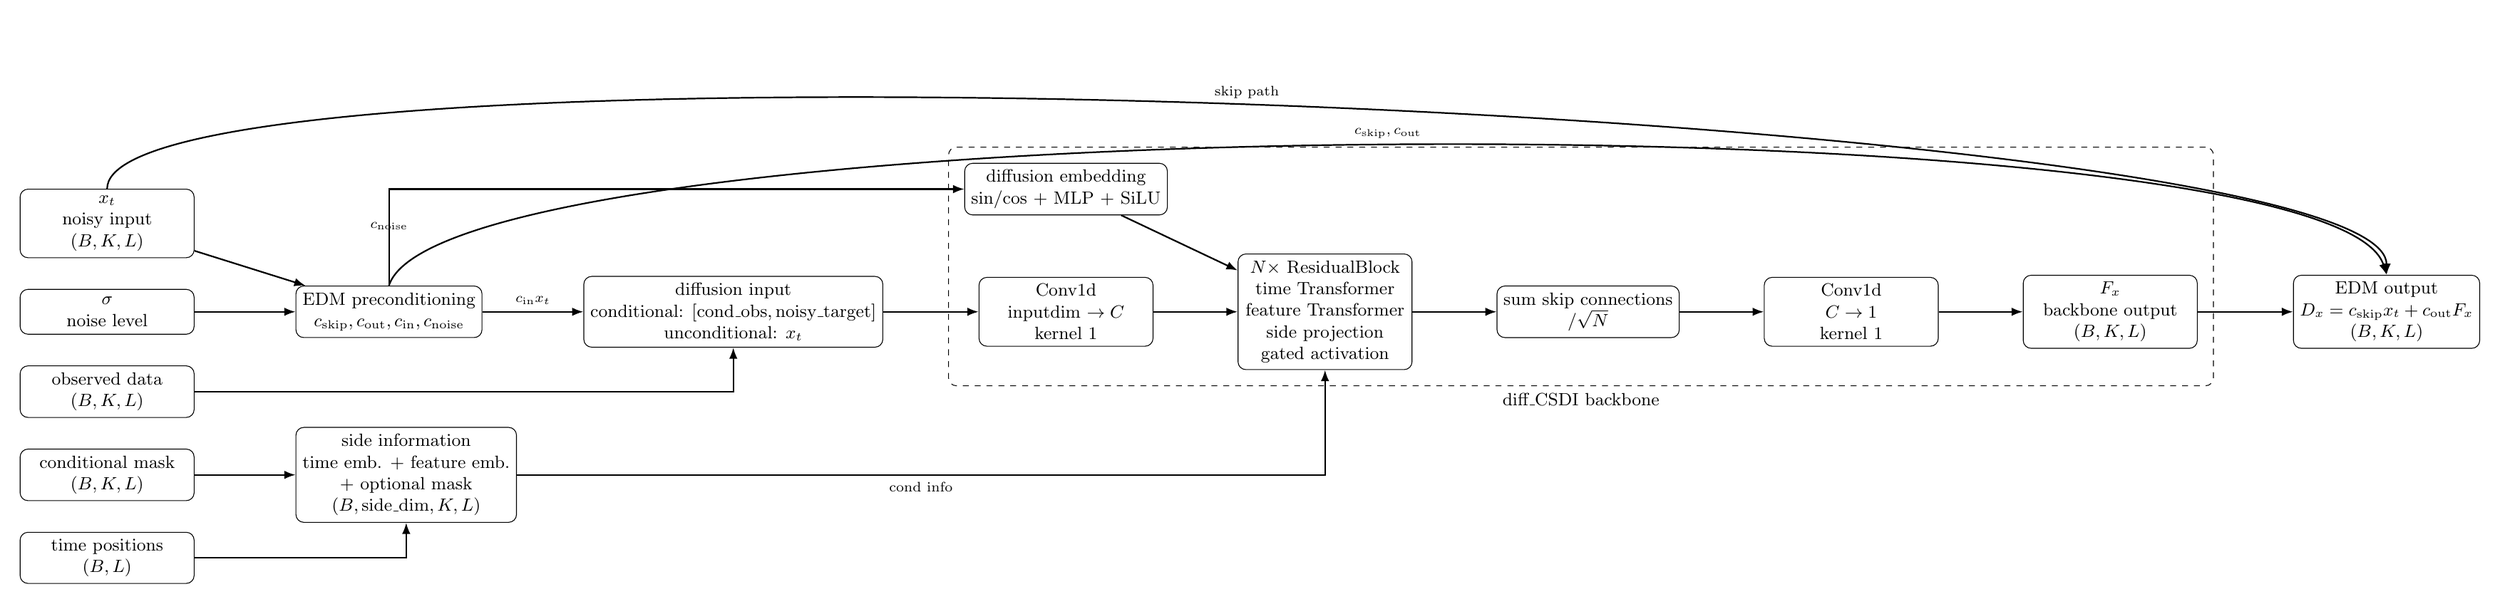
\begin{tikzpicture}[
    block/.style={
        draw,
        rounded corners,
        align=center,
        minimum width=3.1cm,
        minimum height=0.8cm,
        font=\small
    },
    smallblock/.style={
        draw,
        rounded corners,
        align=center,
        minimum width=2.6cm,
        minimum height=0.65cm,
        font=\scriptsize
    },
    arrow/.style={-{Latex[length=2mm]}, thick},
    dashedbox/.style={draw, dashed, rounded corners, inner sep=8pt}
]

% Inputs
\node[block] (xt) {$x_t$\\noisy input\\$(B,K,L)$};
\node[block, below=0.55cm of xt] (sigma) {$\sigma$\\noise level};
\node[block, below=0.55cm of sigma] (obs) {observed data\\$(B,K,L)$};
\node[block, below=0.55cm of obs] (mask) {conditional mask\\$(B,K,L)$};
\node[block, below=0.55cm of mask] (time) {time positions\\$(B,L)$};

% EDM
\node[block, right=1.8cm of sigma] (edm) {EDM preconditioning\\
$c_{\rm skip}, c_{\rm out}, c_{\rm in}, c_{\rm noise}$};

% Side info
\node[block, right=1.8cm of mask] (side) {side information\\
time emb. + feature emb.\\
+ optional mask\\
$(B,\mathrm{side\_dim},K,L)$};

% Diff input
\node[block, right=1.8cm of edm] (diffinput) {diffusion input\\
conditional: $[\mathrm{cond\_obs}, \mathrm{noisy\_target}]$\\
unconditional: $x_t$};

% Backbone
\node[block, right=1.7cm of diffinput] (inconv) {Conv1d\\inputdim $\rightarrow C$\\kernel 1};
\node[block, above=1.1cm of inconv] (diffemb) {diffusion embedding\\sin/cos + MLP + SiLU};

\node[block, right=1.5cm of inconv] (res) {$N \times$ ResidualBlock\\
time Transformer\\
feature Transformer\\
side projection\\
gated activation};

\node[block, right=1.5cm of res] (skip) {sum skip connections\\$/\sqrt{N}$};
\node[block, right=1.5cm of skip] (outconv) {Conv1d\\$C \rightarrow 1$\\kernel 1};
\node[block, right=1.5cm of outconv] (fx) {$F_x$\\backbone output\\$(B,K,L)$};

% Output
\node[block, right=1.7cm of fx] (dx) {EDM output\\
$D_x = c_{\rm skip}x_t + c_{\rm out}F_x$\\
$(B,K,L)$};

% Arrows
\draw[arrow] (xt) -- (edm);
\draw[arrow] (sigma) -- (edm);
\draw[arrow] (edm) -- node[above, font=\scriptsize] {$c_{\rm in}x_t$} (diffinput);

\draw[arrow] (obs.east) -| (diffinput.south);
\draw[arrow] (mask.east) -- (side.west);
\draw[arrow] (time.east) -| (side.south);

\draw[arrow] (diffinput) -- (inconv);
\draw[arrow] (edm.north) |- node[pos=0.25, above, font=\scriptsize] {$c_{\rm noise}$} (diffemb.west);
\draw[arrow] (diffemb) -- (res);
\draw[arrow] (side.east) -| node[pos=0.25, below, font=\scriptsize] {cond info} (res.south);

\draw[arrow] (inconv) -- (res);
\draw[arrow] (res) -- (skip);
\draw[arrow] (skip) -- (outconv);
\draw[arrow] (outconv) -- (fx);
\draw[arrow] (fx) -- (dx);
\draw[arrow] (xt.north) .. controls +(0,3) and +(0,3) .. node[above, font=\scriptsize] {skip path} (dx.north);
\draw[arrow] (edm.north) .. controls +(1,3.2) and +(-1,3.2) .. node[above, font=\scriptsize] {$c_{\rm skip},c_{\rm out}$} (dx.north);

\node[dashedbox, fit=(inconv)(diffemb)(res)(skip)(outconv)(fx),
      label=below:{\small diff\_CSDI backbone}] {};

\end{tikzpicture}
\end{document}